\chapter{Project Time Plan}
\label{ch:Project Time Plan}

\section{TIMEPLAN}
In this section we shall discuss the timeplan, which provides an overview of different tasks and what we would be as a team achieving for the course of one year. The intension of this timeline is to provide a rough idea over the tasks and their times, the actual plan shall be decided and defined as we proceed further during the project. For better understanding, we have divide the project into seven main tasks as shown in the below table.

\begin{table}
\centering
	\begin{tabular}{|c|c|c|c|}
	\hline
		Sr.No. & Tasks & Start & End\\
		\hline
		1 &	Project organization & 11.10.2018 &	10.11.2018\\
		\hline
		2 &	Preparation and Presentation of mini seminar & 11.10.2018 &	19.11.2018\\
		\hline
		3 &	Developing Project Plan & 20.11.2018 & 10.01.2019\\
		\hline
		4 &	Reviewing Technologies & 20.11.2018 & 10.01.2019\\
		\hline
		5 &	Designing Architecture &	06.12.2018 & 10.03.2019\\
		\hline
		6 & Implementation and Deployment &	07.02.2019 & 15.08.2019\\
		\hline
		7 & Presentation &	01.08.2019 & 20.09.2019\\
		\hline
	\end{tabular}
\caption{List of all tasks in the timeplan}
\end{table}
The following list further defines the tasks: 
\begin{enumerate}
	\item \textbf{Project organization:}
	The goal of this task to establish communication between team members so that they can understand each other, in terms of their skills set and expertise. Also decide upon tools for project management, task management, version control and a platform for all further communications.
	\item \textbf{Preparation and Presentation of mini seminar:}
	The goal of this task is to get an overview of various technologies and subjects that is required for the project. Select one of the subjects, research the subject in depth and present the importance of the subject towards project to rest of the team.
	\item \textbf{Developing project plan:}
	The goal of this task is to combine all the subjects presented by each team member and make a basic sketch of what to achieve in the project group, how to achieve it and by when to achieve it. For our project group, the document is a valuable mean to get an overview over the overall problem, related technologies and required subtasks. 
	\item \textbf{Reviewing technologies:}
	The goal of this task is to list all the technologies relevant for the project and to review pros and cons of each the technology and to decide upon technologies to be used in the project.
	\item \textbf{Designing architecture:}
	The goal of this task is to describe in detail and in precise manner on how we are going to achieve the defined tasks and produce end product of the project. This phase is one of the most crucial phase in project group, as it is a core foundation to the project.
	\item \textbf{Implementation and Deployment:}
	The goal of this task is to divide the project group into various sub-groups and each sub-group working independently to produce a stable product by the end of the implementation phase. This can the most effort and time, as we might to develop various versions/prototypes until we obtain an end product that is satisfying and stable. 
	\item \textbf{Presentation:}
	After implementing the system, we will present it to our supervisors and professor. For that, we are going to simulate some use cases and exemplary traffic on a running instance of our software.
	\end{enumerate}

\begin{figure}[h]
\centering
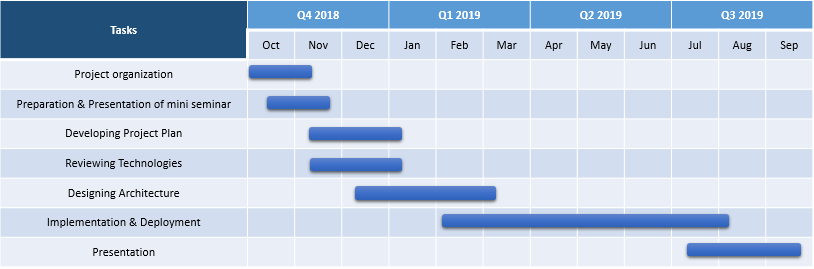
\includegraphics[scale=.6]{timeplan}
\caption{A gantt diagram visualising the timeplan.}
\end{figure}
The sequence of this tasks is visualized in the above diagram. Though the timeline mentioned is fixed and can changes during the course of various phases of project but this is to constantly remind us of the deadlines and to foresee further responsibilities and milestones to be achieved. 


	